\documentclass[sigplan]{acmart}

%New command for paragraphs
\newcommand{\adparagraph}[1]{\paragraph{#1}\mbox{}\\\noindent}

%Command for Markov chain 4
\usepackage{xspace}
\newcommand{\MC}{$\text{MC}_4$\xspace}

%Fixes the style of the ACM article template 
\settopmatter{printacmref=false} % Removes citation information below abstract
\renewcommand\footnotetextcopyrightpermission[1]{} % removes footnote with conference information in first column
\pagestyle{plain} % removes running headers

%Graph packages
\usepackage{tikz}
\usepackage{pgfplots}

%appendix setup
\usepackage{booktabs} % For formal tables
\usepackage[titletoc,toc,title]{appendix}

%note setup
\usepackage{xargs} 
\usepackage{xcolor}
\usepackage[colorinlistoftodos,prependcaption,textsize=tiny]{todonotes}
\newcommandx{\note}[2][1=]{\todo[linecolor=red,backgroundcolor=red!25,bordercolor=red,#1]{#2}\xspace}

% Copyright
\setcopyright{none}
%\setcopyright{acmcopyright}
%\setcopyright{acmlicensed}
%\setcopyright{rightsretained}
%\setcopyright{usgov}
%\setcopyright{usgovmixed}
%\setcopyright{cagov}
%\setcopyright{cagovmixed}
\usepackage{lineno}


\begin{document}
%\linenumbers
\title{Beyond Average}
%\titlenote{Produces the permission block, and copyright information}
\subtitle{Aggregation Methods for Group Based Recommendation Systems}
%\subtitlenote{The full version of the author's guide is available as \texttt{acmart.pdf} document}

\author{Lasse Drustrup Christensen}
%\authornote{}
\affiliation{%
  \institution{Department of Computer Science \\ Aalborg University}
  \streetaddress{Selma Lagerl\"{o}fs Vej 300}
  \city{Aalborg East} 
  \state{Denmark} 
  \postcode{9220}
}
\email{ldch11@student.aau.dk}

\author{Lukas Nic Dalgaard}
%\authornote{}
%\orcid{}
\affiliation{%
  \institution{Department of Computer Science \\ Aalborg University}
  \streetaddress{Selma Lagerl\"{o}fs Vej 300}
  \city{Aalborg East} 
  \state{Denmark} 
  \postcode{9220}
}
\email{lnda12@student.aau.dk}

\author{\textbf{Supervisor}\\ Peter Dolog}
\affiliation{\institution{Department of Computer Science \\ Aalborg University}}
\email{dolog@cs.aau.dk}

% The default list of authors is too long for headers}
%\renewcommand{\shortauthors}{B. Trovato et al.}


\begin{abstract}
In this paper we worked on the problem of recommending items to a group of people based on the preferences of the individual users. We approached this problem as a rank aggregation problem and focused on the top-k preferences of the users.
The methods used for the aggregations were Borda Count, Markov Chain, Spearman's Footrule, and Average.

One of our primary goals were to present a testing setup to give a satisfying theoretical conclusion on which aggregation method to use. For the setup we used Borda Count and Markov Chain showed promising results, but Borda Count was the best performing method.
\end{abstract}

\keywords{Group Recommendation, Rank Aggregation, Borda Count, Markov Chain, Spearman's Footrule, Average, nDCG, Kendall Tau Distance, Spearman's Footrule Distance}
{
    %set up various length
    \ifx\titlepageleftcolumnwidth\undefined{}
      \newlength{\titlepageleftcolumnwidth}
      \newlength{\titlepagerightcolumnwidth}
    \fi
    \setlength{\titlepageleftcolumnwidth}{0.46\textwidth-\tabcolsep}
    \setlength{\titlepagerightcolumnwidth}{\textwidth-2\tabcolsep-\titlepageleftcolumnwidth}
    %create title page
    \thispagestyle{empty}
    \noindent%
    \begin{tabular}{@{}ll@{}}
      \parbox{0.97\titlepageleftcolumnwidth}{
          
\includegraphics[width=0.97\titlepageleftcolumnwidth]{aau_logo_en}
      } &
      \vspace{1cm}
      \parbox{0.97\titlepagerightcolumnwidth}{\raggedleft\sffamily\small
        \textbf{\color{sectioning}Department of Computer Science}\\
        Selma Lagerlöfs Vej 300\\
        DK-9220 Aalborg Ø\\
        \href{http://www.cs.aau.dk}{http://www.cs.aau.dk}
      }\bigskip\\
        \parbox[t]{\titlepageleftcolumnwidth}{
        \textbf{\color{sectioning}\sffamily{Title:}}\\ \projecttitle{}\bigskip\par
        \textbf{\color{sectioning}\sffamily{Theme:}}\\ \projecttheme{}\bigskip\par
        \textbf{\color{sectioning}\sffamily{Project period:}}\\ \projectperiod\bigskip\par
        \textbf{\color{sectioning}\sffamily{Project group:}}\\ \groupname{}\bigskip\par
        \textbf{\color{sectioning}\sffamily{Participants:}}\\ \groupmembersbyfirstname{}\bigskip\par
        \textbf{\color{sectioning}\sffamily{Supervisor:}}\\ \supervisor\bigskip\par
        \textbf{\color{sectioning}\sffamily{Copies:}} \projectcopies\bigskip\par
        \textbf{\color{sectioning}\sffamily{Pages:}}~\pageref*{LastPageLabel}\bigskip\par
        \textbf{\color{sectioning}\sffamily{Date of completion:}}\\ \projectcompletion
  } &
      \parbox[t]{0.97\titlepagerightcolumnwidth}{%
      \textbf{\color{sectioning}\sffamily{Abstract:}}\smallskip\par{}
        \fbox{\parbox{0.97\titlepagerightcolumnwidth-2\fboxsep-2\fboxrule}{%
          Group recommendation, while plagued by the inability to obtain an optimal satisfaction for all members, is still improvable. In this report the group recommendations are based on rank aggregation, mainly Borda Count, and voting systems, in the form of Single Transferable Vote. These new approaches are combined to form what we dubbed Borda Transferable Count, a method that our preliminary tests show to give the group about 12\% more satisfaction than the classic rank aggregation method of Borda.
        }}
      }\\
    \end{tabular}
    \vfill
      \noindent{\footnotesize\emph{The content of this report is freely available, but publication (with reference) may only be pursued due to agreement with the authors.}}
    \clearpage
  }

\begin{titlepage}
\section*{Summary}
\note{Write me}

\end{titlepage}
\maketitle

\section{Introduction}
Many of the decisions we make are based on recommendation, from either people we know or a recommender system which knows our preferences, due to the amount of information overload we are exposed to. The recommendations, or more specific on our case the recommender system, can be a help to reduce the amount of information we are presented with to a manageable level and hereby ease the decision making without forcing a decision on us. 

The problem with the traditional recommender systems is that it typically make recommendations specifically to one person put often these decisions needs to be taken in a social context. Some scenarios where this could be the case is for example selecting a film to watch from the seemingly endless ones available on the streaming services, Which restaurant you should go to, or which vacation destination suits you best. 

One for the problem regarding taking the social context into consideration is that the recommender have to strive for consensus between the people it recommends to. From here, we will reference to this problem as making a group recommendation.

%Different methods for group recommendations 
When making group recommendations there are two main approach namely profile aggregation and recommendation aggregation.\note{cite, page 516 in rec. book} The idea behind profile aggregation is to aggregate the users preferences into a group profile and make aggregations based on that profile. The recommendation aggregation method aggregates the recommendations for the individual users into one aggregation that should fit the groups preferences. In this paper we have chosen to focus on the latter, as we want to make the method work for shifting groups and we deem this approach to fit this case best. \note{find source or fitting argument}

%Describe the approach of using top-k lists 
As we are going to aggregate the users recommendations we have chosen to only to focus at the top-k part of their recommendations and return a top-k lists as a result. Furthermore, the top-k lists will be ranked with the highest rated item at first position on the list. Throughout the paper we have worked with a $k$ of size 10. 

Working with partial lists, which ranked top-k lists are, we have selected three types of aggregation list which have shown good results when used for aggregating search engine results within the information retrieval domain. The methods we are using is Borda Count, Markov Chain, and Spearman's Footrule. We also implemented an Average aggregation method as a control algorithm. 

%Problem regarding evaluation of the aggregation results
Having the group recommendations we are faced with the challenge of evaluating the result as there are no dataset supplying us with a ground truth. Alternatively we use some different equality measures in order to verify the results. 
\note{extend this}


%Lukas
%As it is no longer of question of should the computers be involved when humans make decisions but how.

%Recommender systems can strengthen decision making without taking away the final choice from humans. This opens the 

%For making a decision, Edwards et al provide a 19 step guide for picking the option with the highest utility, and they argue that the problem for a user would be in picking from among the many options presented, also known as information overload\cite{Edwards2001}.

%Recommender systems deal with reducing the problem for a user to a manageable amount of choices. Given a user's preferences, a good recommender system can narrow down the number of choices to a manageable level.

%However when the problem area is expanded to include multiple users in need of a single choice, the problem area is two-fold, as the many individual preferences must be aligned into that of a single recommendation.

%The recommender system is doubly challenged as while a single user can navigate the given recommendations and reflect on each item for the best optimal choice, a group will have a hard time making insightful decisions about items they lack the shared information of the group to comment on.
\note{Lukas: Possible direction for the introduction?}

\subsection{Composition of a Group Recommender}
As we take the aspect of aggregating recommendations the group recommendation system will consist of two parts namely an individual recommender and an aggregation method. \note{need some extension and probably an illustration}

\subsection{Thesis}\note{Placeholder title}
How can we by supplying a rank aggregation method with an array ranked top-k lists $\tau_1, ... , \tau_u$, where $u$ is the number of group members, get a recommendation performing better than an average aggregation. \note{this should probably be more specific and technical}

\subsection{Structure of the Paper}
The structure of the paper is as follows. In Section \ref{sec:preliminaries} contains the preliminaries including the measures used during the evaluation. Section \ref{sec:aggregations} describes the aggregation methods used. In Section \ref{sec:evaluation} the performances of the aggregation methods are documented. Section \ref{sec:discussion} we discuss the results of the evaluation and in Section \ref{sec:conclusion} we will present our conclusion and some future work to be done.
\section{System Overview}\label{sec:systemoverview}
In this section we give a short overview of the group recommendation system which is depicted in Figure \ref{fig:composition}. Each of the stages will be outlined with a short description. 
\begin{figure}[H]
\centering
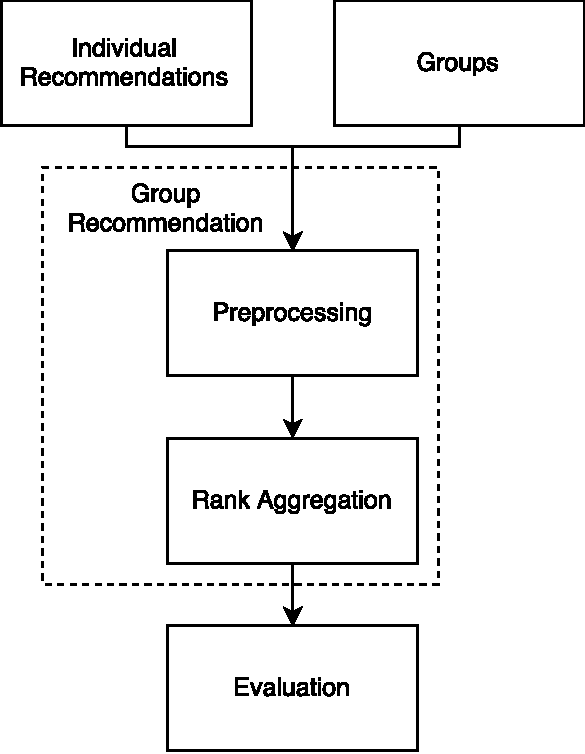
\includegraphics[scale=.4]{graphics/composition}
\caption{Stages of the group recommender system}\label{fig:composition}
\end{figure}
\paragraph{Individual Recommendation} We make individual recommendations for every user. The recommendation methods used in this step is interchangeable and can be selected to fit the data and purpose of the recommendation. The only condition for the recommender is that it finds a complete list of recommendations of the users in a group. In Section \ref{sec:individualrecommender} the recommender we use is further elaborated on.

\paragraph{Groups} In the groups stage we generated a list of groups for testing purposes. These groups consist of user id's and were generated at random but it is ensured that the same user only appears once in each group. The specific setup of the groups is described in Section \ref{sec:groupgeneration}.

\paragraph{Group Recommendation} The group recommendation part consists of two stages, namely preprocessing and rank aggregation.
\begin{itemize}
\item Preprocessing is needed to find the individual recommendations belonging to the users in a certain group and format them for the rank aggregation.
\item Rank aggregation combines the individual recommendations into a list of size $k$ which should represent the groups preferences.
\end{itemize}
A more detailed description of the stages in group recommendation can be found in Section \ref{sec:grouprecommendation}.
%\paragraph{Preprocessing} Before being able to aggregate the ratings preprocessing is needed. The preprocessing step takes a group as input and is concerned with finding the $k$ highest rated items for each of the users in the group. The items are arranged in a ranked lists with the highest rated item first and descending. The lists are stored in an array. A more detailed explanation of the preprocessing can be found in the introduction to Section \ref{sec:aggregations}.

%\paragraph{Aggregation} In the aggregation stage a selection of different aggregation methods was implemented and was interchangeable with each other. All the methods took the array of lists, which was supplied from the preprocessing stage, as input. The output of the aggregations is the group recommendation in the form of a ranked list of size $k$. In the subsections of Section \ref{sec:aggregations} are a description of the aggregation methods. 

\paragraph{Evaluation} The last stage is evaluation. In this stage several tests and measurements are performed. The setup and results of this stage is shown in Section \ref{sec:evaluation}.


%As we are going to aggregate recommendations we implemented a group recommender system with the steps shown in Figure \ref{fig:composition}. A dataset will provide for us to make some individual recommendations for users arranged into groups for later testing. The next part of the group recommender is the aggregation half, which is the focus of the paper. Using the output of the first part of the system, we will be trying several different aggregation approaches. The results of these are the group recommendations to be evaluated.
%As we take the aspect of aggregating recommendations the group recommendation system will consist of two parts namely an individual recommender and an aggregation method. \note{need some extension and probably an illustration}

%\section{Preliminaries}\label{sec:preliminaries}
This section provides some preparatory knowledge about the setup of the recommender system, ranked lists, and the satisfaction and distance measures.
\subsubsection{Dataset}\label{sec:dataset}
We used the MovieLens 100k dataset published by GroupLens in 1998\cite{movielens100k}. MovieLens 100K contains 100.000 ratings between 1 to 5 collected from 943 users across 1682 movies. With room for approximately one and a half million ratings, the 100k rating dataset is sparse. We used rating prediction to populate the rating matrix.

\subsubsection{Individual Recommendations}\label{sec:individualrecommendation}
For rating prediction, we used the library called MyMediaLite\cite{mymedialite}. MyMediaLite is a library for .NET that holds a bundle of recommendation methods for both item recommendation and rating prediction. We will be using the library, because this gives a tested foundation that is easy to reproduce for testing other aggregation methods and the focus of our paper lies in testing the aggregation methods.

Among the methods provided by MyMediaLite, SVD++ is one of the best performing on the 100k dataset on their own records using the parameters in Table \ref{tbl:svdpp}\footnote{www.mymedialite.net/examples/datasets.html}. For the sake of convenience we are using the same parameters as they are proven to be efficient.

\begin{table}[H]
	\centering
	\begin{tabular}{|l|l|}\hline
		Latent Factors & 50 \\
		Regularization & 1	\\
		Bias Regularization & 0.005	\\
		Learning Rate & 0.01 \\
		Bias Learning Rate & 0.07 \\ 
		Number of iterations & 50 \\
		Frequency Regularization & True \\\hline
	\end{tabular}
	\caption{Parameters values for the SVD++ component}
	\label{tbl:svdpp}
\end{table}

\subsubsection{Group Generation}\label{sec:groupgeneration}
For the aggregation we made groups consisting of 4, 8, 12, 16, 20, and 40 users from the MovieLens 100K dataset. This allows us to further the findings by Baltrunas et al\cite{Baltrunas:2010:GRR:1864708.1864733}, who had group sizes from 2 to 8.

Given that the dataset contains 943 users, we limited our group size to 40, as to not have any groups containing more than 5\% of all the users. This ensured some amount of diversity in the group. 40 is also ten times the size of our smallest group, enough to indicate the trend for the quality of recommendations. The groups were created of randomly picked users, and the same user can appear in multiple groups, but never in the same group twice.
\subsubsection{Ranking Measures}\label{sec:ranking}
\note{Make an introduction, old intro was ranking.}
%\subsubsection{Satisfaction Measures}
%\adparagraph{nDCG}

\begin{figure}[H]
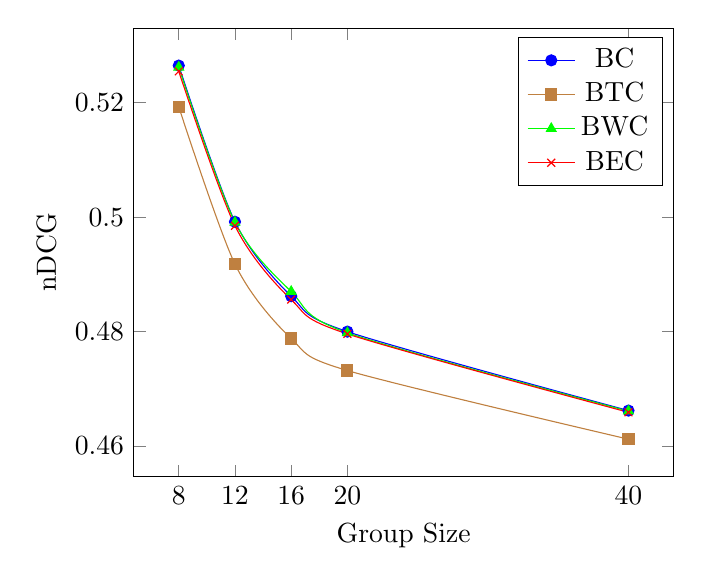
\begin{tikzpicture}
\begin{axis}[
	xlabel=Group Size,
	ylabel=nDCG,
	xtick = {4,8,12,16,20,40}]
		\addplot[smooth,mark=*,blue] plot coordinates {
		%(4,0.6028)
		(8,0.5265)
		(12,0.4992)
		(16,0.4862)
		(20,0.48)
		(40,0.4662)
	};
	\addlegendentry{BC}
	
	\addplot[smooth,color=brown,mark=square*] plot coordinates {
		%(4,0.5995)
		(8,0.5193)
		(12,0.4918)
		(16,0.4788)
		(20,0.4732)
		(40,0.4612)
	};
	\addlegendentry{BTC}
	
	
	\addplot[smooth,color=green,mark=triangle*] plot coordinates {
		%(4,0.6022)
		(8,0.5262)
		(12,0.4991)
		(16,0.487)
		(20,0.4798)
		(40,0.4661)
	};
	\addlegendentry{BWC}
	
	
	\addplot[smooth,color=red,mark=x] plot coordinates {
		%(4,0.6010)
		(8,0.5255)
		(12,0.4985)
		(16,0.4856)
		(20,0.4796)
		(40,0.4659)
	};
	\addlegendentry{BEC}

\end{axis}
\end{tikzpicture}
\caption{Results using nDCG on BC extensions}\label{fig:appendixndcg}
\end{figure}
\subsubsection{Distance Measures}\label{sec:distance}
Before going through the distance measures, we want to cover some general notations that both methods use. As we work with comparing two top-k lists, which are partial lists, we denote them as $\tau_1$ and $\tau_2$. $\tau_1 (i)$ is the notation for the position of element $i$ in $\tau$. $Z = \tau_1 \cap \tau_2$, $z=|Z|$, $S$ is the set of items in $\tau_1$ but not $\tau_2$ and $T$ is vice versa, and $k$ is the length of the top-k lists.

\adparagraph{Kendall Tau Distance}
The idea of Kendall tau distance(KTD) is to compare two ranked lists based on the order in which the items appear. This basically means that it makes pairwise comparisons of item indexes $\{i,j\}$ where $i < j$, so that if $i$ is before $j$ in $\tau_1$ then this should also be the case in $\tau_2$ in order to get a good score. The score is based on a count of how many times $i$ and $j$ are in reverse order. The equation for KTD for complete lists can be seen in Equation \ref{eq:kendalldistancefinal} where $K_1$ and $K_2$ can be seen in Equation \ref{eq:kendalldistance1} and \ref{eq:kendalldistance2} respectively.

\begin{equation}\label{eq:kendalldistance1}
K_1(\tau_1,\tau_2) = | \{(i,j) | i < j, \tau_1 (i) < \tau_1 (j) \land \tau_2 (i) > \tau_2 (j)\}|
\end{equation}
\begin{equation}\label{eq:kendalldistance2}
K_2(\tau_1,\tau_2) = | \{(i,j) | i < j, \tau_1 (i) > \tau_1 (j) \land \tau_2 (i) < \tau_2 (j) \} |
\end{equation}
\begin{equation}\label{eq:kendalldistancefinal}
K(\tau_1,\tau_2) = K_1(\tau_1,\tau_2) + K_2(\tau_1,\tau_2)
\end{equation}

In order to adjust KTD for partial lists we used the $K_{Haus}$ algorithm proposed by Fagin et al\cite{comparing:topk}. This approach has four different cases.

The first case is when both $i$ and $j$ appear in $\tau_1$ and $\tau_2$. In this case the method utilizes Equation \ref{eq:kendalldistancefinal} but only on the items in the set, $Z$.

The second case is when $i$ and $j$ both appear in $\tau_1$ or $\tau_2$ but only $i$ or $j$ appears in the other. Case two is calculated according this formula $(k-z)(k+z+1)- \sum_{i \in S} \tau_1(i)- \sum_{i \in T} \tau_2(i)$. The formula takes the maximum number of items and subtracts the positions from the list containing the items.\note{Revise this explanation, as it is more complex.}

Third case is when $i$ appears in one list and $j$ in the other. For these cases the distance is measured as $(k-z)^2$, which is the disjunctive union of both lists to the power of 2.

The fourth case is when both $i$ and $j$ appear in one list but not the other. In this case Equation \ref{eq:case4} is used. $p$ in this case is a penalty value between 0 and 1. As the method we use is an average approach this value is naturally 0.5. $p$ is multiplied with the binomial coefficient of the length of different items in the top-k lists.

\begin{equation}\label{eq:case4}
2p\left(\!
    \begin{array}{c}
      k-z \\
      2
    \end{array}
  \!\right)
\end{equation}


Combining these cases into one method, we get the $K_{Haus}$ algorithm which can be seen in Equation \ref{eq:khaus}. 
\footnotesize
\begin{equation}\label{eq:khaus}
K_{Haus}(\tau_1,\tau_2) = \frac{1}{2}(k-z)(5k-z+1)+ \sum_{i,j \in Z} K_{i,j}(\tau_1,\tau_2) + \sum_{i \in S}\tau_1(i) - \sum_{i \in S}\tau_1(i)
\end{equation}
\normalsize

The result of the $K_{Haus}$ is normalized by dividing it by $n(n-n)/2$, which gives an approximation of the average distance between the lists. It is an approximation because in case four, the method assumes that there is an equally large chance of the items being in the correct order. Due to this, the method returns 0.78 if the lists are completely disjoint. If the lists are reverse of each other it scores 1 and 0 if the lists are equal. %For a more detail explanation of $K_{Haus}$ go to Fagin et al\cite{comparing:topk} article.

 
\note{Mention somewhere that the results are averages of all group members and all groups}

\adparagraph{Spearman's Footrule Distance}
Another distance measure we use is the Spearman's Footrule Distance(SFD). SFD finds the exact distance between item $i$ in two different ranked lists containing $i$. The way it finds this item distance is by subtracting the item indexes from each other as can be seen in \ref{eq:sfd}. 

\begin{equation}\label{eq:sfd}
F(\tau_1, \tau_2) = \sum_{i=1}^{k} | \tau_1 (i) - \tau_2 (i) |
\end{equation}

As we work with partial lists we use an alternate version called $F_{Haus}$, see Equation \ref{eq:fhaus}, proposed by Fagin et al\citep{comparing:topk}.
As the lists $\tau_1$ and $\tau_2$ can contain different items, the missing index values for items are replaced by $\ell$ which is some value larger than $k$, as it follows that they would be outside the top-k list. Based on the article by Fargin et al we set $\ell$ to be equal to $(3 * k - z + 1)/2$.

\footnotesize
\begin{equation}\label{eq:fhaus}
F_{Haus}(\tau_1,\tau_2)= (k-z)(3k-z+1)+\sum_{i\in Z} | \tau_1 (i) - \tau_2 (i) | - \sum_{i\in S} \tau_1 (i) - \sum_{i\in Z} \tau_2(i)
\end{equation}
\normalsize
% some items will be missing on the lists. In order to handle this we insert $\ell$ which is equal to $(3 * k - z + 1)/2$ placing the item \note{find reason}.  

In order to normalize we divide the result of Equation \ref{eq:fhaus} by $n^2 /2$ which is the maximum value of the algorithm. Doing so we get a value of 0 if $\tau_1$ and $\tau_2$ are in the same order or 1 if the lists are the reverse of each other or completely disjoint.
\section{Group Recommendation}\label{sec:grouprecommendation}
This section documents the preprocessing done and outlines the rank aggregation methods used in order make the recommendation aggregation into a group recommendation. 
%In this section we explain the workings and concept behind the four aggregation methods.

\subsection{Preprocessing}
Prior to making the rank aggregation we do some preprocessing. As specified in Figure \ref{fig:composition} the preprocessing stages get groups and all the individual recommendations as input. Preprocessing is concerned with constructing a top-k list for each of the users in a specific group based on the individual recommendations.

A top-k list is specified as a ranked list of length $k$ consisting of the highest rated items order in descending order. More specifically let $\tau$ be a top-k list and let $\tau(i)$ be the rating of item $i$, which is an arbitrary item, then list is ranked if $\tau (1) > \tau (2) > ... > \tau (k)$.

The top-k lists are stored in a array which is used as input for the aggregation methods.

\subsection{Rank Aggregation}\label{sec:aggregations}
In this section we describe the aggregation methods. Common for all the aggregation methods is that they aggregate an array of top-k lists into one ranked list, $\omega$, of length $k$ containing recommendations of a group which is returned. The order of $\omega$ may differ between the methods as they rank it based on which items they deem most relevant for the group with the most relevant item first. 

\begin{frame}[t]
\frametitle{Borda Count}
\begin{columns}
\begin{column}{0.5\textwidth}
\begin{align*}
	bc(i) = \sum_{u\in U} \tau_u(i)
\end{align*}
\small
\begin{align*}
	bc(A) = \tau_{u_1}(A) + \tau_{u_2}(A) + \tau_{u_3}(A) + \tau_{u_4}(A)
\end{align*}
\normalsize
\begin{align*}
	bc(A) = 5 + 4 + 2 + 3 = 14
\end{align*}

\end{column}
\begin{column}{0.5\textwidth}
\small
\vspace{-0.5cm}
\begin{table}
\captionsetup{font=footnotesize}
\begin{tabular}{|l|lllll|} \hline
Rank  & 1 & 2 & 3 & 4 & 5 \\\hline
$u_1$ & A & B & C & D & E \\
$u_2$ & C & D & F & A & E \\
$u_3$ & E & A & G & B & D \\
$u_4$ & G & H & A & E & F\\\hline
\end{tabular}
\caption{Top-k list of a group with 4 users}
\end{table}

\vspace{-1cm}
\begin{table}
\begin{tabular}{|l|llllllll|}\hline
      & A & B & C & D & E & F & G & H \\\hline
$u_1$ & 5 & 4 & 3 & 2 & 1 & 0 & 0 & 0 \\
$u_2$ & 2 & 0 & 5 & 4 & 1 & 3 & 0 & 0 \\
$u_3$ & 4 & 2 & 0 & 1 & 5 & 0 & 3 & 0 \\
$u_4$ & 3 & 0 & 0 & 0 & 2 & 1 & 5 & 4 \\\hline
Sum	  & 14& 6 & 8 & 7 & 9 & 4 & 8 & 4 \\\hline
\end{tabular}
\caption{Borda Count scores}
\end{table}
\normalsize
\end{column}
\end{columns}
\begin{table}
\begin{tabular}{llllll}
Recommendations: & A & E & C & G & D
\end{tabular}
\end{table}
\end{frame}

%
%\begin{columns}
%\begin{column}{0.5\textwidth}
%
%\end{column}
%\begin{column}{0.5\textwidth}
%
%\end{column}
%\end{columns}
\subsection{Markov Chain}\label{sec:markovchain}
The proposed Markov Chain method by Dwork et Al, \MC is a generalization of the Copeland Method\note{find cite for this}, where a winner is the candidate which wins the most pairwise contests\citep{rank:aggregation}.

The concept behind building the list of recommendations works by explicitly finding the transition matrix. For \MC, the states are connected to other states that wins per the Copeland method. Then we can iterate through the set, and note who performs best to make the transition matrix. Using the power set on the transition matrix we can find the stationary probability distribution to aggregate the candidates.

The \MC state space corresponds to a set of all the items ranked. The corresponding transition matrix for \MC will have an equal chance of transitioning to any other state that can beat it in a majority of pairwise contests.

Given partial lists $\tau_1,...,\tau_k$, collectively known as $\tau$, with rankings of items, and the state space, $S$, of \MC corresponding to the set of all items ranked in those partial lists. If the current state is item $i$ we can transition to uniformly picked state $j \in S$ where $j$ is ranked higher than item $i$ on a majority of lists in $\tau$ which ranked both $i$ and $j$. Otherwise, we stay in state $i$.

%Non-strict markov chain
\MC as presented by Dwork et al is used on metasearch and aggregating query results, whereas we work in the recommendation domain. To better suit our domain, we make a small adjustment to the method. For search engine comparison, partial lists might not contain both items needed for a pairwise comparison, so in the event of only one item being on the list, it is unknown if the other search engines have ranked the item or not, so Dwork et al restrict themselves to the pairwise comparisons available, and rely on the connectivity in the chain to correct any outcomes.

For our domain we have estimated the rankings giving us a top-k of a full list. So we follow this line of thinking for partial lists containing neither of the items, as the highest rank is not available. However, if the partial list contains one of the items, it wins that pairwise contest, as the losing item is known to be somewhere down the list.

%$p_{ij} = Pr(X_{n+1} = \sum_{l=1}^{k} \tau_l(i) < \tau_l(j) | X_n = \sum_{l=1}^{k} \tau_l(i) > \tau_l(j) )$

%Strict markov chain
%For completeness, we also tested a stricter interpretation of \MC where only the majority winners with both items present were considered.
\subsection{Spearman Footrule}\label{sec:spearmanfootrule}
\subsection{Average}\label{sec:average}
As a control algorithm we choose Average(Avg) aggregation as it is one of the more common used and well performing methods within group recommendation.\note{cite} The implementation we have done does only work with the items in the top-k list. It finds the union of all the users $u\in U$ lists so $\tau_1 \cup ... \cup \tau_u = I$. The Avg method then uses the full lists, $\sigma_1, ..., \sigma_u$, from the individual recommendations to find the average rating for the items $i \in I$. Equation \ref{eq:avg} illustrates how Avg works.

\begin{equation}\label{eq:avg}
Avg(i) = \frac{\sum_{u \in U} \sigma_u(i)}{|U|} 
\end{equation}
\note{ u in U doesn't stand under sum}
\section{Evaluation}

\subsubsection{Dataset}\label{sec:dataset}
We used the MovieLens 100k dataset published by GroupLens in 1998\cite{movielens100k}. MovieLens 100K contains 100.000 ratings between 1 to 5 collected from 943 users across 1682 movies. With room for approximately one and a half million ratings, the 100k rating dataset is sparse. We used rating prediction to populate the rating matrix.

\subsubsection{Individual Recommendations}\label{sec:individualrecommendation}
For rating prediction, we used the library called MyMediaLite\cite{mymedialite}. MyMediaLite is a library for .NET that holds a bundle of recommendation methods for both item recommendation and rating prediction. We will be using the library, because this gives a tested foundation that is easy to reproduce for testing other aggregation methods and the focus of our paper lies in testing the aggregation methods.

Among the methods provided by MyMediaLite, SVD++ is one of the best performing on the 100k dataset on their own records using the parameters in Table \ref{tbl:svdpp}\footnote{www.mymedialite.net/examples/datasets.html}. For the sake of convenience we are using the same parameters as they are proven to be efficient.

\begin{table}[H]
	\centering
	\begin{tabular}{|l|l|}\hline
		Latent Factors & 50 \\
		Regularization & 1	\\
		Bias Regularization & 0.005	\\
		Learning Rate & 0.01 \\
		Bias Learning Rate & 0.07 \\ 
		Number of iterations & 50 \\
		Frequency Regularization & True \\\hline
	\end{tabular}
	\caption{Parameters values for the SVD++ component}
	\label{tbl:svdpp}
\end{table}

\subsubsection{Group Generation}\label{sec:groupgeneration}
For the aggregation we made groups consisting of 4, 8, 12, 16, 20, and 40 users from the MovieLens 100K dataset. This allows us to further the findings by Baltrunas et al\cite{Baltrunas:2010:GRR:1864708.1864733}, who had group sizes from 2 to 8.

Given that the dataset contains 943 users, we limited our group size to 40, as to not have any groups containing more than 5\% of all the users. This ensured some amount of diversity in the group. 40 is also ten times the size of our smallest group, enough to indicate the trend for the quality of recommendations. The groups were created of randomly picked users, and the same user can appear in multiple groups, but never in the same group twice.
\subsection{Discussion} \label{sec:discussion}

Across all the methods tested we saw a similar fall in nDCG scores and distance for the distance measures as group size increased, except for some methods in Rating nDCG.

We also saw a trend of the nDCG score being a good indicator for how well the same  methods performed for the distance measure. Though SF performs well in SFD, but it falls behind on other measures, with the same to be said for Avg and its performance for Rating nDCG. This stresses the importance of testing a general purpose method from many angles.

Across all the measurements, \MC is almost identical in performance to that of BC. As the underlying heuristic of the \MC method is the Copeland Method, it raises the possibility that other extensions of Markov Chain can achieve even greater results.

However for \MC, other factors such as complexity and speed limits the utility of it compared to BC, as BC is both simple to implement and can be implemented in linear time whereas \MC time complexity is a little more tricky\citep{rank:aggregation}.\note{Time complexity of \MC}

Of all the measures, Avg has the worst results overall, depending on how Rating nDCG is viewed. The results from Rating nDCG in isolation sees Avg perform the best. So if Rating nDCG is a better measurement because it does not consider the rankings, and instead looks directly at the ratings given by the users, then Avg is providing the better recommendations. However, in such a scenario, the difference between Avg and its nearest competitor is so small that there is little practical value to gain. Should it be the case that Rating nDCG is the best measure, we have a theory about rearranging the users top-k list and order them according to average. We will expand on this in future work in Section \ref{sec:futurework}.

Overall, the best performing method for our tests is BC, as it consistently exceeds or matches the other methods.

%All methods saw similar decreases in effectiveness across group sizes.

%BC performed best for nDCG. Other benefits include fast computation time, simple to implement. Outperforms or stands equal to various extensions we've developed. Compared with MC for nDCG, the mean difference is small, but consistent.

%MC performed 2nd best for nDCG. Our implementation is very slow, but it can be optimized a lot (probably still not faster than BC). No indication in data, but might surprise for bigger topK lists, which in turn raises the connectivity (main strength). Runs on the Copeland method, which is ill regarded for aggregation, but works reasonably well here.

%Avg generally performs poorly. It gets some good results in Adjusted nDCG, but that is a measurement uniquely advantageous for it among the methods, so it makes little sense as a measure.

%X method is the best

%When to use kendall and nDCG? For our results, it's not that important.
\chapter{Conclusion} \label{ch:conclusion}
We wanted to showcase an approach that reconciles the differences in preferences among multiple group members in the problem of group recommendation. During this process we found that the evaluation possibilities of the performance of these approaches were rather limited due to lack of proper datasets making it difficult to determine whether or not a group would be satisfied with its recommendations.

We found that with using a ranked list for the recommendations we could adopt the normalized Discounted Cumulative Gain(nDCG) technique from the information retrieval domain to measure user satisfaction by comparing the ranked list of a user with the ranked list found through aggregation. This only left us with the task of forming the groups, which we ended up doing using random sampling.

We sought to answer the following questions from the problem statement:
\begin{itemize}
	\item How to reflect group decision making algorithmically while securing satisfaction for the individuals as well as the group as a whole?
	\item How to measure the level of satisfaction in a group in regards to the items recommended?
	\item How to make recommendations to a group of people based on the users' individual preferences?
\end{itemize}

For reflecting how a group decision would be handled, we ventured into some of the methods used for resolving differing opinions. In the end, we incorporated single transferable vote into the Borda Count method in the Borda Transferable Count(BTC) algorithm. These are not methods that necessarily reflects an organic group decision process, but reflects parts of real group decision methodologies.

For measuring the level of satisfaction in a group, we found and used nDCG. It is commonly used for rankings and information retrieval. This works well with the view of recommendation as a tool for drawing out relevant information, when getting an overview is hard.

For making recommendations to a group, we present the BTC as a method of aggregating the individual ranked lists. The results are promising, as it performs better than the tested methods on nDCG scores. However, we cannot as of yet make a definite conclusion on the BTC as a solution to the group recommender problem.

\section{Discussion}\label{sec:conclusion_discussion}
As mentioned we use the information retrieval method nDCG to measure satisfaction. In doing so we make several assumptions about the users’ preferences. First of all, the user ratings used for the group recommendations are predictions, which may not coincide with the actual preferences of the user. Based on these predicted ratings we assume that a user would construct a ranked list, with a fixed distance between the top ranked and next highest rank regardless of the predicted preference for either, which we use to determine the satisfaction score, with the highest ratings. This means that the satisfaction score we get is based on assumptions about a user's preferences, which makes our results noteworthy, but ultimately, based on assumptions about existing data rather than real world data.

In order for us to get a concrete result we need to measure satisfaction with real users as to prove the effectiveness of the method presented in this project. Provided that, the method could point in the direction that group recommendation is a voting problem.
\section{Acknowledgements}\note{To be written}

%AAU
%Claus

%Should co-author Peter Dolog be here?

\bibliographystyle{ACM-Reference-Format}
\bibliography{references} 

\newpage

\begin{appendices}
\section{Survey}
%Context about why we needed the data

%How the whole thing went down
In order to make a dataset in a short time frame, we looked into crowdsourcing, where it was possible to pay people to answer surveys or do tasks that computers cannot. In particular we were looking at Clickworker and Mechanical Turk, which allowed external surveys. Since no sites had an inbuilt survey creation tool that could handle our requirements, we decided to make our own survey website.

Using this method, we could potentially reach thousands of people without limiting us to the survey tools made available on the standard websites.

%Creation of the website
For web hosting, we went to DigitalOcean, which offered a Ubuntu server setup with Django. We added Gunicorn as the WSG interface and nginx as the http server. Behind it all, we had a MySql database keeping track of the survey questions and results along with timestamps.

%Django as Python web application framework
%Gunicorn as Web Server Gateway Interface(WSGI) server. A traditional web server does not understand or have any way to run Python applications. WSGI is a standard interface for py modules and containers.
%Digical Ocean as webhost with Unix as the OS
%MySql as the database

%The survey
The survey itself asks participants to personally give a recommendation to a group of users. The participant knows each user's own top 10 preference, and must decide on their own what aggregation strategy they wish to follow. An important aspect of the survey was making it as easy to complete as possible. As we had to pay each participant, each such improvement could be translated to a saving, which in turn translated to a larger and more useful dataset. So to make it more intuitive and not overload each user with information, we made it so that hovering the mouse over a movie title will make the movie's position light up on all the other users' rankings, shown in Figure \ref{fig:appendix_userprefs}, and gave the user a tooltip about other movie positions. Additionally, we made the ranking system into a drag-and-drop, such that the participant could drag and easily rearrange their recommendations. This can be seen in Figure \ref{fig:appendix_recbox}.

\begin{figure}\label{fig:appendix_recbox}
	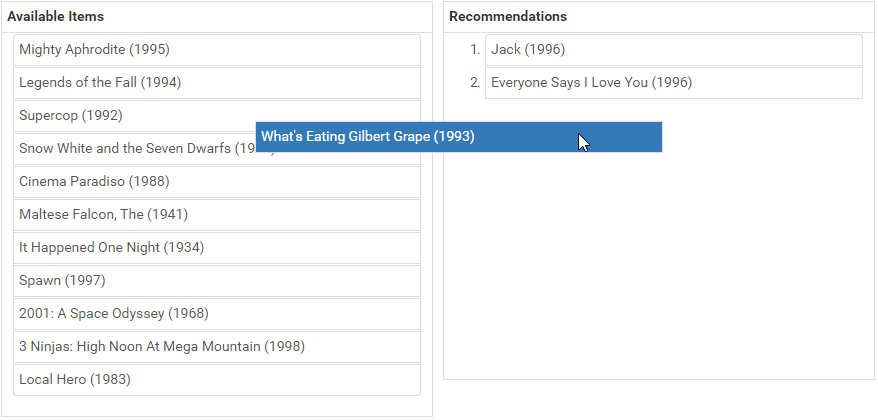
\includegraphics[scale=0.35]{graphics/recbox.png}
	\caption{The list of available items and the box holding the recommendations of the survey participant}
\end{figure}

\begin{figure}\label{fig:appendix_userprefs}
	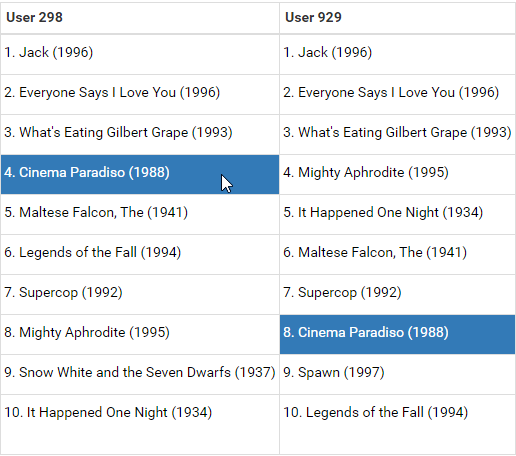
\includegraphics[scale=0.5]{graphics/users.png}
	\caption{Two lists of movie preferences for a user}
\end{figure}

After making a recommendation, the user could proceed to the next step, and upon completing all steps they would reach a screen providing them with a code. With each step, the group size is increased by one, going from 4 to 8 users. The code is important, as the participant must present this as evidence to the crowdsourcing site as proof of their participation. For our survey, we decided to generate a unique code for each participant mixing the assigned groups and a timestamp, so that we could deduce which user responded when and with what. This precaution was necessary so that it was possible to filter out participants rushing through the survey with no care for their answers.

Also, since we wanted to have a balanced dataset, we separated our groups into 40 sets of groups of size 4 to 8, and made it so that every user would get a randomly picked set. The database would keep track of how many responses each set had, such that we could prioritize the sets with fewer responses and get a balanced dataset. It would also mean that anyone taking the test twice would be unlikely to see the same survey.

Before running the survey on Mechanical Turk, we ran it past some other willing participants for evaluation and decided to halve the number of groups each participants would give recommendations to from 10 to 5, due to feedback about the length of the survey. \note{This section can be expanded to better reflect the process and changes happening to the survey, as a lot of work went into it in the project}

%Most importantly, we realized how vital it was to make the par

%Dealing with mechanical turk
For the crowdsourcing website, we ended up going with Amazon's Mechanical Turk, as it is the more well-known and cheaper service. When ready, we injected a good amount of money on the account, as one had to prepay for any work requested and started up a limited run to test out the services and find a suitable price range. We managed to get a few responses. On Mechanical Turk, the participant would see our survey, click in and be provided a link to our survey. Upon completion of the survey, our participant would get the code and input it on the Mechanical Turk website. Initial results were interesting with big differences between how much time participants spent on the survey. We noted a few obvious cheaters who blazed through a survey in seconds thanks to the timestamps, however as a requester and with the timestamps in our database, we would be able to sort them out, and we could also reject their work on the Mechanical Turk site.

Though, on the third day of this limited run we ran into problems with Amazon Mechanical Turk. We were unable to access our account, and had to contact their support team. Soon enough the support team responded that our account had been suspended, and that we would be informed about the reason for the suspension in 2-3 days along with fate of our account. In two days time, Mechanical Turk support wrote us that our account had been suspended indefinitely and our current survey stopped because of a violation of the participation agreement. Unaware of any possible violations we could have made, we made further inquires, but never got a clear answer. Additionally, our funds on the account were also confiscated. So in the end, we ended up only getting responses totaling a few dollars worth of data.

%Show data and evaluate on them.
\end{appendices}

\end{document}
